\section{Agent}

\begin{cstqsn*}
What is an \textbf{agent}?
\end{cstqsn*}

Anything that can be viewed as 

\begin{enumerate}
  \item Perceiving its environment through sensors; and 
  \item Acting upon that environment through actuators.
\end{enumerate}

\begin{cstqsn*}
What is a \textbf{rational agent}?
\end{cstqsn*}

A rational agent will choose an action that is expected to maximize its
performance measure, given the evidence provided by: 

\begin{itemize}
  \item the \textbf{percept sequence}; and 
  \item the \textbf{built-in knowledge} it has.
\end{itemize}

\begin{cstqsn*}
When do we say that an agent is \textbf{autonomous}?
\end{cstqsn*}

If its behavior is determined by its own experience.

\begin{cstqsn*}
What is the \textbf{PEAS} framework?
\end{cstqsn*}

\begin{itemize}
  \item Performance Measure 
  \item Environment 
  \item Actuators 
  \item Sensors
\end{itemize}

\section{Characterizing the environment}

\begin{cstqsn*}
When do we say that an environment is \textbf{fully observable} (v.s. partially
observable)?
\end{cstqsn*}

An agent's sensors give it access to the complete state of the environment at
each point in time.

\begin{cstqsn*}
When do we say that an environment is \textbf{deterministic} (v.s. stochastic)?
\end{cstqsn*}

The next state of the environment is completely determined by the current state
and the action executed by the agent.


\begin{cstqsn*}
When do we say that the environment is \textbf{strategic}?
\end{cstqsn*}

If the environment is \textbf{deterministic} except for the actions of other
agents, then the environment is strategic.

\begin{cstqsn*}
When do we say that the environment is \textbf{episodic} (v.s. sequential)?
\end{cstqsn*}

The agent's experience is divided into atomic ``episodes", where each episode
consists of the agent perceiving and then performing a single action. 

The choice of action in each episode depends only on the episode itself.

\begin{cstqsn*}
When do we say that the environment is \textbf{static} (v.s. dynamic)? When do
we say that the environment is \textbf{semi-dynamic}?
\end{cstqsn*}

The environment is \textbf{unchanged} while an agent is deliberating. 

The environment is \textbf{semi-dynamic} if the environment itself does not
change with the passage of time but the agent's performance score does.

\begin{cstqsn*}
When do we say that a environment is \textbf{discrete} (v.s. continuous)?
\end{cstqsn*}

When there are a \textbf{limited} number of \textbf{distinct}, \textbf{clearly
defined} percepts and actions.

\begin{cstqsn*}
When do we say that the environment is \textbf{single-agent} (v.s. multi-agent)?
\end{cstqsn*}

When an agent is operating by itself in an environment.

\section{Models for Agent Organization}

\begin{cstqsn*}
What are the five models for agent organization?
\end{cstqsn*}

\begin{enumerate}
  \item Simple reflex agents;
  \item Model-based reflex agents;
  \item Goal-based agents;
  \item Utility-based agents;
  \item Learning agents.
\end{enumerate}

\subsection{Simple Reflex Agents}

\begin{cstqsn*}
What is a \textbf{simple reflex agent}? What is the agent function based on?
\end{cstqsn*}

Simple reflex agents \textbf{ignore} the rest of the percept history and act 
only on the basis of the current percept. 

The agent function is based on the \textbf{condition-action rule}.

\begin{center}
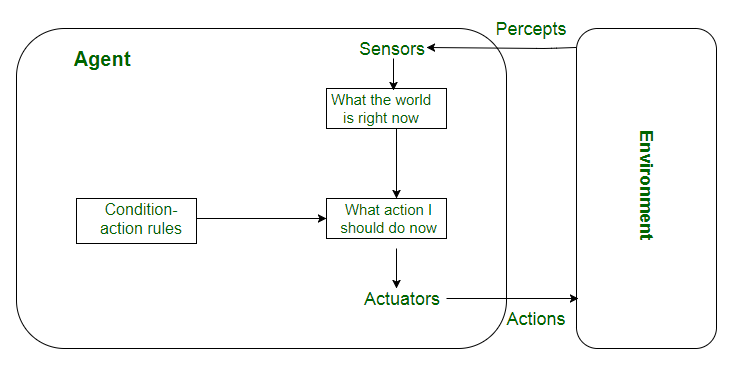
\includegraphics[width=0.8\textwidth]{images/lec01/simple_reflex_agent.png} 
\end{center}

\begin{cstqsn*}
What is the \textbf{percept history}?
\end{cstqsn*}

It is the history of all that an agent has perceived to date.

\begin{cstqsn*}
What are the \textbf{downsides} of a \textbf{simple reflex agent}?
\end{cstqsn*}

\begin{itemize}
  \item Very limited intelligence.
  \item No knowledge of non-perceptual parts of the state.
  \item Usually too big to generate and store.
  \item If there occurs any change in the environment, then the collection of
    rules need to be updated.
\end{itemize}

\subsection{Model-Based Reflex Agents}

\begin{cstqsn*}
What is a \textbf{model-based reflex agent}? How does it work?
\end{cstqsn*}

A model-based reflex agent works by finding a rule whose condition matches the
current situation.

\begin{center} 
  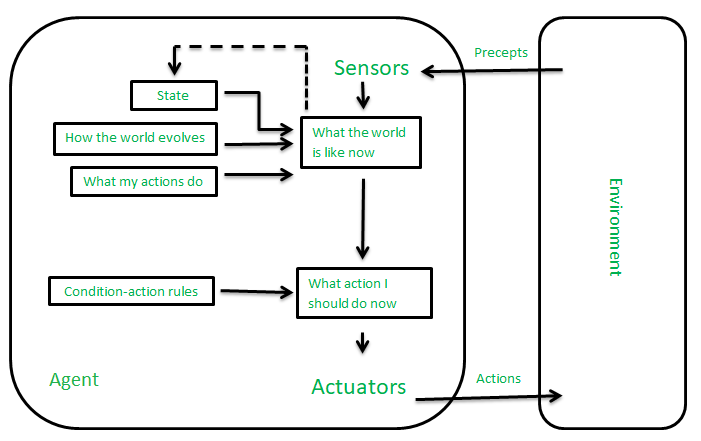
\includegraphics[width=0.8\textwidth]{images/lec01/model-based_reflex_agent.png}
\end{center}

\begin{cstqsn*}
Can a model-based agent handle partially observable environments?
\end{cstqsn*}

Yes, it can, by \textbf{the use of a model about the world}.

\begin{cstqsn*}
What does \textbf{model-based reflex agent} do to its percepts?
\end{cstqsn*}

It keeps track of the \textbf{internal state}, which is adjusted by each
percept and that depends on the percept history.

\begin{cstqsn*}
How does a \textbf{model-based reflex agent} update its \textbf{internal
state}? (i.e. what two pieces of information does it need?)
\end{cstqsn*}

\begin{itemize}
  \item How the world evolves independently from the agent; and 
  \item How the agent's actions affect the world.
\end{itemize}

\subsection{Goal-based agents}

\begin{cstqsn*}
What are \textbf{goal-based agents}? How do they make decisions?
\end{cstqsn*}

Goal-based agents make decisions based on \textbf{how far they are currently
from their goal}. Their every action is intended to reduce its distance from
the goal.

\section{Exploitation and Exploration}

\begin{cstqsn*}
What is the \textbf{trade-off between exploitation and exploration}?
\end{cstqsn*}

An agent in operating in the real world must often choose between: 

\begin{itemize}
  \item Maximizing its expected utility according to its current knowledget
    about the world;
  \item trying to learn more about the world.
\end{itemize}
